\documentclass[11pt]{article}

% ---------------------------------------------------------------------------
%  Fixed polyplets: a(19), hole stratification, and generating functions
%  (OEIS A006770 and companions)
% ---------------------------------------------------------------------------
\usepackage[margin=1in]{geometry}
\usepackage{amsmath,amssymb}
\usepackage{booktabs}
\usepackage{graphicx}
\usepackage{numprint}
\usepackage{microtype}
\usepackage[hidelinks]{hyperref}
\usepackage{flafter}   % a float never appears before the text that introduces it
\usepackage{float}     % [H] pins tables/figures exactly where written
\usepackage[font=small,labelfont=bf,labelsep=period]{caption}  % captions visually distinct from body
\setlength{\intextsep}{16pt plus 3pt minus 3pt}  % a little more breathing room

% comma thousands-separator, grouping 4-digit numbers too; \num is an alias so
% the body can stay package-agnostic.
\npthousandsep{,}
\npfourdigitsep
\newcommand{\num}[1]{\numprint{#1}}
\newcommand{\byH}{\ensuremath{B_H}}

\title{\textbf{Fixed polyplets: $a(19)$ and $a(20)$, hole stratification,
and generating functions}\\[2pt]
\large Two confirmed new terms of OEIS A006770, with new hole-count sequences and
exact fixed-height generating functions}
\author{Jason Parker \texttt{<jasonp@panix.com>}\\[2pt]
\small Independent researcher (unaffiliated)}
\date{June 2026}

\begin{document}
\maketitle

\begin{abstract}
\noindent
A \emph{polyplet} (king-move animal) is a finite set of unit cells of the square
lattice connected through shared edges or corners. OEIS sequence
\href{https://oeis.org/A006770}{A006770} counts the \emph{fixed} polyplets of $n$
cells, until now known through $n=18$. We report two new terms,
\[
  a(19) = \num{151609203011580},\qquad a(20) = \num{1025573519362016},
\]
both computed from scratch and reproducing all eighteen prior terms. The first is
confirmed by two algorithms that share no counting logic---decorrelated Redelmeier
enumeration and a column transfer matrix; $a(20)$, beyond Redelmeier's reach, is
confirmed by independent recomputation on a second architecture together with exact
generating-function cross-checks. We extend the free, one-sided, and symmetry-typed
companions to $n=20$ (A030222, A030233, A030234/A030235), and develop further
results the same machinery yields: a
hole-count stratification of A006770 (a new triangle whose hole-free and one-hole
columns are absent from OEIS), exact rational generating functions at each fixed
bounding-box height, the extremal maximum hole \emph{area} ($\sim n^2/8$), and
rigorous lower bounds on $a(n)$ with a uniform-sampling portrait. Results computed
and validated but not proved are labeled as such; all code, data, and a
claim-verifier are released.
\end{abstract}

\section{Introduction}
\label{sec:intro}

The enumeration of lattice animals---finite connected sets of cells on a regular
lattice---is a classical problem at the meeting point of combinatorics and
statistical physics~\cite{klarner,jensen2001}. On the square lattice the two
standard families are \emph{polyominoes}, connected through shared edges, and
\emph{polyplets}, connected through shared edges or corners. The fixed counts grow
exponentially, so exact values are known only for modest $n$ and each new term is
a small computational milestone. The fixed-polyomino sequence
(\href{https://oeis.org/A001168}{A001168}) has been pushed
furthest~\cite{redelmeier,jensen2003,barequet}; the fixed-polyplet sequence
A006770 had been recorded through $n=18$.

This note reports and confirms the next term, $a(19)$, and then develops several
further results about polyplets that the same machinery yields: the
hole-stratified counts (Section~\ref{sec:holes}), exact fixed-height generating
functions (Section~\ref{sec:gf}), and a sampling/scaling portrait with rigorous
bounds (Section~\ref{sec:sampling}). It is an amateur contribution carried out
with substantial AI assistance (Section~\ref{sec:ai}); its value lies not in
algorithmic novelty but in independent, cross-checked computation. Since a single
$15$-digit count from one program is properly a conjecture, $a(19)$ is computed
twice, by two algorithms that share no counting logic, on different hardware and
compilers, both reproducing the entire published range.

\section{Definitions}
\label{sec:object}

Fix the square lattice $\mathbb{Z}^2$ and call its unit squares \emph{cells}. A
\emph{lattice animal} is a finite, nonempty, adjacency-connected set of cells.
Under \textbf{rook} (edge) adjacency the animals are \emph{polyominoes}; under
\textbf{king} (edge-or-corner) adjacency they are \emph{polyplets}. Every
polyomino is a polyplet but not conversely: two cells touching only at a corner
form a polyplet and not a polyomino (Figure~\ref{fig:specimen}). One subtlety: a
polyplet connected \emph{purely} by diagonals lives on a single checkerboard
colour class, itself a square lattice, so such a shape is a polyomino in disguise.
A genuinely king shape mixes edge and corner contacts.

Animals are counted \textbf{fixed} (up to translation; rotations and reflections
distinct), \textbf{one-sided} (up to translation and rotation), or \textbf{free}
(up to all isometries). A006770 is the fixed count.

\begin{figure}[H]
  \centering
  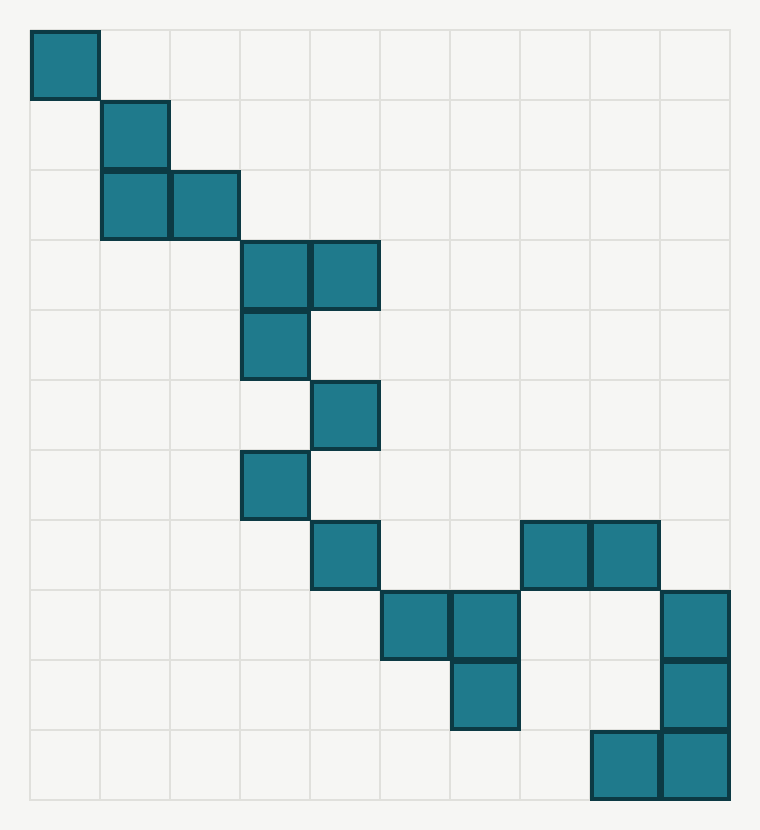
\includegraphics[width=0.36\textwidth]{../results/a19_specimen.png}
  \caption{A $19$-cell fixed polyplet (drawn uniformly at random; bounding box
  $11\times 10$). Under rook adjacency it splits into nine pieces, so the diagonal
  corner-contacts alone hold it together---a polyplet, not a polyomino.}
  \label{fig:specimen}
\end{figure}

\section{The count and its companions}
\label{sec:result}

\begin{equation}
  \boxed{\,a(19) = \num{151609203011580},\quad a(20) = \num{1025573519362016}\,}
\end{equation}

The full sequence is in Table~\ref{tab:terms}; terms $n\le 18$ reproduce A006770
exactly and $n=19,20$ are new. The growth ratios $a(19)/a(18)\approx 6.7468$ and
$a(20)/a(19)\approx 6.7646$ continue the slow climb of successive ratios toward the
king-lattice growth constant; ratio extrapolation over $n=10,\dots,20$ gives
$\lambda\approx 7.10$ with critical exponent $\theta\approx-1$, consistent with the
universal value for two-dimensional lattice animals~\cite{jensen2001} (a heuristic
series estimate, not a bound).

\begin{table}[H]
  \centering
  \small
  \begin{tabular}{r r @{\quad}|@{\quad} r r}
    \toprule
    $n$ & $a(n)$ & $n$ & $a(n)$\\
    \midrule
    1  & \num{1}              & 11 & \num{39299408}\\
    2  & \num{4}              & 12 & \num{257105146}\\
    3  & \num{20}             & 13 & \num{1692931066}\\
    4  & \num{110}            & 14 & \num{11208974860}\\
    5  & \num{638}            & 15 & \num{74570549714}\\
    6  & \num{3832}           & 16 & \num{498174818986}\\
    7  & \num{23592}          & 17 & \num{3340366308393}\\
    8  & \num{147941}         & 18 & \num{22471158811164}\\
    9  & \num{940982}         & \textbf{19} & $\mathbf{\num{151609203011580}}$\\
    10 & \num{6053180}        & \textbf{20} & $\mathbf{\num{1025573519362016}}$\\
    \bottomrule
  \end{tabular}
  \caption{Fixed polyplets $a(n)$, $n=1,\dots,20$. Terms $1$--$18$ match the
  published A006770; $a(19)$ and $a(20)$ are the new terms.}
  \label{tab:terms}
\end{table}

\paragraph{Companions.}
Counting the same cells under coarser equivalences gives the free, one-sided, and
symmetry-typed companions, all from the fixed count by Burnside's lemma over the
square's symmetry group $D_4$:
\[
  \mathrm{Free}=\tfrac18(\mathrm{Fixed}+2R_{90}+R_{180}+2H+2D),\qquad
  \mathrm{OneSided}=\tfrac14(\mathrm{Fixed}+2R_{90}+R_{180}),
\]
where $R_{90},R_{180},H,D$ count the animals fixed by a $90^\circ$ rotation, a
$180^\circ$ rotation, an axis reflection, and a diagonal reflection, from a
dedicated enumerator over fundamental domains. At $n=19$ these are $R_{90}=0$ (a
$90^\circ$-symmetric animal needs $n\equiv0,1\pmod4$, but $19\equiv3$),
$R_{180}=\num{10178520}$, $H=\num{9765524}$, and $D=\num{8923786}$.

The resulting counts for $n=18,19,20$ are collected in Table~\ref{tab:companions}.
The free and one-sided values extend A030222 and A030233 (each previously recorded
to $n=17$); the bilaterally-symmetric count $\tfrac12(H+D)$ extends A030234 and the
asymmetric count $\mathrm{Free}-\tfrac12(H+D)$ extends A030235.

The bilateral count equals $\tfrac12(H+D)$ exactly, by a double count. Write the
symmetry group of a fixed polyplet as a subgroup $K\le D_4$. If $K$ contains a
reflection, its rotations form an index-$2$ subgroup, so exactly half of $K$'s
elements are reflections; otherwise $K$ has none. Count the incidences $(A,m)$ of a
fixed animal $A$ with a reflection $m\in\operatorname{Stab}(A)$ in two ways. Summed
over the four reflections it is
$|\!\operatorname{Fix}(h)|+|\!\operatorname{Fix}(v)|+|\!\operatorname{Fix}(d)|
+|\!\operatorname{Fix}(a)| = 2H+2D$, since conjugate reflections have equal
fixed-counts ($|\!\operatorname{Fix}(h)|=|\!\operatorname{Fix}(v)|=H$,
$|\!\operatorname{Fix}(d)|=|\!\operatorname{Fix}(a)|=D$). Summed over free classes, a
class with stabilizer order $|K|$ contains $8/|K|$ fixed animals, each with $|K|/2$
reflections in its stabilizer when the class is bilateral (and none otherwise)---so
exactly $4$ incidences per bilateral class. Hence $2H+2D=4\cdot(\text{bilateral
classes})$, i.e.\ the bilateral count is $\tfrac12(H+D)$. This was also checked
numerically against every published term of A030234 ($n\le17$).

As a check, the assembled free counts reproduce A030222 over its entire published
range, and an independent Python reimplementation matches the C\texttt{++}
symmetric sub-counts at $n=19$.

\begin{table}[H]
  \centering\small
  \resizebox{\textwidth}{!}{%
  \begin{tabular}{l r r r l}
    \toprule
    count & $n=18$ & $n=19$ & $n=20$ & OEIS\\
    \midrule
    fixed                 & \num{22471158811164} & \num{151609203011580} & \num{1025573519362016} & A006770\\
    free                  & \num{2808898025438}  & \num{18951156321090}  & \num{128196711128365}  & A030222\\
    one-sided             & \num{5617792259411}  & \num{37902303297525}  & \num{256393397108358}  & A030233\\
    bilaterally symmetric & \num{3791465}        & \num{9344655}         & \num{25148372}         & A030234\\
    asymmetric            & \num{2808894233973}  & \num{18951146976435}  & \num{128196685979993}  & A030235\\
    \bottomrule
  \end{tabular}}
  \caption{Fixed polyplets and their companions at $n=18,19,20$. A006770 was known
  to $n=18$ and the companions to $n=17$, so every $n=19,20$ entry (and the
  companions' $n=18$) is new.}
  \label{tab:companions}
\end{table}

\section{Method A: direct enumeration}
\label{sec:methodA}

Redelmeier's backtracking enumeration~\cite{redelmeier}, adapted to king
adjacency, grows every animal exactly once from an anchored cell: it maintains an
ordered frontier of \emph{untried} neighbours and recurses, with the standard
rule that a cell once placed or rejected at a level is excluded from deeper
levels. The recursion tallies by size; no animal is stored. Being embarrassingly
parallel by sub-tree, the count was run as two decorrelated campaigns---on
\texttt{gympie} (Apple silicon, Apple~clang, frontier split $7\times64$) and
\texttt{ayr} (AMD Threadripper, GCC/x86, split $8\times96$). The per-size outputs
are \textbf{byte-identical} (SHA-256 \texttt{558f0bdf\ldots}). Because the two
campaigns differ in hardware, compiler, and scheduling and the arithmetic is exact
integer addition, a transient or platform-specific fault in one is overwhelmingly
unlikely to be mirrored digit-for-digit in the other; the error mode they cannot
jointly catch is a bug in the shared \emph{algorithm}, which is what Method~B
rules out.

\section{Method B: the column transfer matrix}
\label{sec:methodB}

The second method counts the same animals by an entirely different principle:
dynamic programming over the connectivity of a moving boundary, with no animal
materialised---a king adaptation of the transfer-matrix / finite-lattice
technique for polyominoes~\cite{jensen2001,jensen2003,bousquet}. Every animal has
a bounding-box height $H$, and animals of height exactly $H$ are counted
separately, so $a(n)=\sum_{H=1}^{n}\byH(n)$ (Table~\ref{tab:byheight}); the
heights are independent, checkpointable sub-problems.

Within a height, confine the animal to an $H$-row strip and sweep columns left to
right. A \emph{boundary signature}---the occupancy of the most recent column, a
partition of its filled cells into the partial animal's connected components, and
two flags for whether rows $0$ and $H-1$ have yet been touched---is a Markov state,
since a future cell attaches only to the current column or later. Because king
adjacency reaches the diagonal neighbours $(c{-}1,r{\pm}1)$, the transfer moves an
\emph{entire column} at once, keeping the previous column wholly present;
connectivity across the step is resolved by union--find. Three invariants make
accepted sweeps biject with fixed polyplets: the first column is column $0$ (no
horizontal double-counting); an animal is tallied only with both touch-flags set
(height exactly $H$); and only when its boundary is a single component---partial
states that can never reconnect are pruned. A size-budget prune drops any state
whose cells-so-far plus an \emph{admissible} lower bound on cells-still-needed
exceeds $n$. Since the bound never over-estimates, the prune can only make a
count come out low, so reproducing every published term certifies that it dropped
no animal in range. The hot path uses a flat open-addressing map keyed by a
fixed-width signature, a stack union--find, and a viable-mask generator.

\begin{table}[H]
  \centering
  \small
  \begin{tabular}{r r @{\quad}|@{\quad} r r}
    \toprule
    $H$ & $\byH(19)$ & $H$ & $\byH(19)$\\
    \midrule
    1  & \num{1}              & 11 & \num{17644523530186}\\
    2  & \num{15994426}       & 12 & \num{11003764277892}\\
    3  & \num{12736006193}    & 13 & \num{5776897734667}\\
    4  & \num{452027455240}   & 14 & \num{2512138867830}\\
    5  & \num{3469435781222}  & 15 & \num{882180009630}\\
    6  & \num{10975452058596} & 16 & \num{240601488426}\\
    7  & \num{20257323484797} & 17 & \num{47839787379}\\
    8  & \num{26611876627714} & 18 & \num{6170030010}\\
    9  & \num{27701775032858} & 19 & \num{387420489}\\
    10 & \num{24014057424024} & & \\
    \midrule
    \multicolumn{4}{r}{$\sum_H \byH(19) = \num{151609203011580}$}\\
    \bottomrule
  \end{tabular}
  \caption{The height decomposition $\byH(19)$ of $a(19)$, peaking at $H=9$. The
  extreme entry is a closed form: a height-$H$ animal of $H$ cells is one cell per
  row drifting by $\{-1,0,+1\}$ at each of $H-1$ steps, so
  $\byH(H)=3^{H-1}$; here $B_{19}(19)=3^{18}=\num{387420489}$.}
  \label{tab:byheight}
\end{table}

\section{Confirmation}
\label{sec:confirm}

The value rests on several independent checks.
\begin{itemize}
  \item \textbf{External truth and Method A $=$ Method B.} Both methods reproduce
        A006770 exactly for every $n\le 18$, and the transfer-matrix totals
        $\sum_H\byH(n)$ are byte-identical to the Redelmeier output (same SHA-256)
        at every term through $n=19$.
  \item \textbf{Forward vs.\ backward DP.} A separate backward completion-count
        DP, run on a different host, compiler, and ISA, reproduced a
        representative height term $B_{17}(19)=\num{47839787379}$ identically.
  \item \textbf{Structural cross-checks.} The transfer matrix's
        (height,\,size) and (size,\,perimeter) marginals match the enumeration's
        through $n=12$. Of the generated polyplets, those connected under rook,
        and bishop, adjacency reproduce A001168, as does the perimeter-$4n$ slice.
  \item \textbf{Fault injection.} Planted errors are caught (a dropped diagonal at
        $n=2$, a doubled count at $n=1$, a prune off-by-one at $n=10$) while a
        provably count-preserving change survives---so the checks fail on wrong
        programs and pass on right ones.
  \item \textbf{Hygiene.} Both engines are AddressSanitizer/UBSan clean; the
        multithreaded transfer matrix is ThreadSanitizer clean and bit-identical
        to the serial path.
\end{itemize}

\section{Hole stratification}
\label{sec:holes}

A \emph{hole} of a polyplet is a bounded connected component of its complement.
For king (8-connected) foreground the topologically consistent choice is
\textbf{4-connected} background: a single diagonal staircase of cells then seals
a region (its corner gaps are not 4-passable), matching the Jordan-curve picture
and the convention of \href{https://oeis.org/A389193}{A389193} for ordinary
polyominoes.

We stratify A006770 by hole count: let $T(n,k)$ be the number of
fixed $n$-cell polyplets with exactly $k$ holes, so $\sum_k T(n,k)=a(n)$.

The column transfer matrix of Section~\ref{sec:methodB} carries $k$ as a second
additive index via the Euler characteristic ($\#\text{holes}=1-\chi$ for a
connected animal, $\chi$ accumulated by local $2\times2$ bit-quad increments~\cite{gray});
the resulting counts are exact, byte-identical to an independent per-animal flood
fill for $n\le14$, and have row sums equal to A006770 (including the confirmed
$a(19)$). These counts are exact through $n=18$; the full triangle is in the repository, and
Table~\ref{tab:holes} lists its first rows. At $n=18$ there are
$A_0(18)=\num{16503616943998}$ hole-free polyplets and $A_1(18)=\num{4970078092354}$
with a single hole, the maximum being $10$.

Independent checks come in two forms. The per-animal flood fill that verifies the
low rows caps at $n=14$; rows $n=15$--$18$ are confirmed instead by a
second-architecture recount (clang/ARM against the GCC/x86 run, byte-identical
across the whole triangle), so no row rests on a single engine.

\begin{table}[H]
  \centering\small
  \begin{tabular}{r r r r r}
    \toprule
    $n$ & $k=0$ & $k=1$ & $k=2$ & $k=3$\\
    \midrule
    4 & \num{109}    & \num{1}     &           & \\
    5 & \num{622}    & \num{16}    &           & \\
    6 & \num{3664}   & \num{166}   & \num{2}   & \\
    7 & \num{22094}  & \num{1456}  & \num{42}  & \\
    8 & \num{135609} & \num{11788} & \num{538} & \num{6}\\
    \bottomrule
  \end{tabular}
  \caption{The hole triangle $T(n,k)$ (number of fixed $n$-cell polyplets with
  exactly $k$ holes; $4$-connected-background convention), rows $n=4$--$8$; full
  data, exact through $n=18$, is in the repository. The hole-free column $k=0$ is
  $1,4,20,109,622,3664,22094,135609,843941,\dots$ and the one-hole column $k=1$ is
  $1,16,166,1456,11788,91300,\dots$ (onset $n=4$); both are absent from OEIS.}
  % TODO(oeis-Anums): the hole triangle T(n,k) and its columns A_0 (hole-free) and
  % A_1 (one-hole) are drafted in oeis/ but not yet submitted/assigned. When OEIS
  % assigns A-numbers, replace "absent from OEIS" here with the live references and
  % add the A-numbers to the data-availability section. Same for M(n) if minted.
  \label{tab:holes}
\end{table}

\paragraph{Maximum hole area.}
How much empty area can $n$ cells enclose? Let $M(n)$ be the maximum number of
enclosed empty cells over all $n$-cell polyplets. A diamond (L$^1$-ball) wall of
$4r$ cells on $|x|+|y|=r$ is king-connected and seals the $2r^2-2r+1$ cells inside
it, so $M(4r)\ge 2r^2-2r+1$ (the centered square numbers,
\href{https://oeis.org/A001844}{A001844}: $1,5,13,25,41,\dots$). This diamond is asymptotically optimal. When the boundary is measured in the king
($L^\infty$, Chebyshev) metric---the line integral of $\max(|dx|,|dy|)$---the
area-maximizing shape is the diamond, the $L^1$ ball dual to the $L^\infty$ square
(Busemann's isoperimetrix~\cite{strang}). Hence $M(n)\sim n^2/8$, twice the
polyomino rate $\sim n^2/16$, since only king animals can run the diagonal walls the
$L^1$ ball requires.

Brute force gives the exact values $M(1{:}16)=0,0,0,1,1,2,3,5,6,8,10,13,15,18,21,25$,
which the diamond attains at $n=4$, $8$, $12$, and $16$ (there $M=1,5,13,25$ meet
$2r^2-2r+1$ at $r=1,2,3,4$); every multiple-of-four term computed so far meets the
diamond bound exactly.

What the isoperimetric bound does not pin down is the \emph{exact} value of $M(n)$
at each $n$: the integer sequence above, its behaviour away from multiples of four,
and whether the diamond is exactly (not just asymptotically) optimal. These remain
open for $n>16$. Extending past
the prior $n=9$ also disambiguates $M(n)$ from the unrelated short OEIS sequences
sharing the prefix $0,0,0,1,1,2,3,5,6$.
% M(n) now exact to n=16 (M(15)=21, M(16)=25; diamond tight at n=16). M(17) (~2.5 days)
% is past the per-term time line, so the sequence stops at n=16 by choice, not capacity.

\section{Generating functions by height}
\label{sec:gf}

For a fixed bounding-box height $H$, the strip transfer matrix has a
bounded state space, so $\byH(n)$ satisfies a finite-order linear recurrence and
its generating function $G_H(x)=\sum_n \byH(n)\,x^n=P_H(x)/Q_H(x)$ is
rational~\cite{stanley}. We
recover these exactly for $H\le10$ by Berlekamp--Massey~\cite{massey} over $\mathbb{Z}/p\mathbb{Z}$
for several primes followed by CRT (lifting past $64$ bits), each accepted only when
the fitted recurrence reproduces held-out terms. The denominators $Q_H$ have
orders\footnote{These orders are $3$-term running sums of \emph{atom} degrees
$1,2,4,9,29,68,181,\dots$: each $Q_H$ factors as $N_{H-2}N_{H-1}N_H$, where $N_H$ is
the denominator of the height-$H$ strip generating function, so every irreducible
factor divides exactly three consecutive $Q_H$. This ``lifetime three'' is a
second-difference effect ($B_H=V_H-2V_{H-1}+V_{H-2}$), universal across finite-range
animal classes and verified here for $H\le7$; neither degree sequence appears in
OEIS.} $1,3,7,15,42,106,278,711,1897,5005$ for $H=1,\dots,10$. Recovering $G_H$ needs
about twice that many series terms; the strip height is fixed, so generating them
costs time but little memory---here it is series length, not the per-state memory
that limits the $a(n)$ computation, that sets the ceiling. We recover all ten (they
are listed in the data release; $G_3$ below is a representative example). The $H=10$
recovery, needing $\sim\!10{,}000$ terms, was itself reproduced on a second
architecture (clang/ARM against the GCC/x86 run, byte-identical), so the GFs are
cross-checked.
As an example,
\[
  G_3(x)=\frac{9x^3-8x^4-2x^5+4x^6+x^7}{1-7x+15x^2-9x^3-3x^4+5x^5-x^6-x^7}.
\]

\paragraph{Hole-resolved.}
Refining by hole count makes each fixed-$(H,k)$ row C-finite as well: $G_{H,k}(x)$
is the $[q^k]$ coefficient of a rational bivariate $G_H(x,q)$, hence rational. A
mod-$p$ version of the hole transfer matrix (counts reduced modulo $p$, with
partial states beyond the target $k$ dropped---exact since holes only seal, never
reopen, as columns are added) yields arbitrarily many terms; we recover $G_{H,k}$
for $H\le6$ (all reachable $k$), the rows $k\le2$ at $H=7$, and the single row $k=0$
at $H=8$, each validated against a fresh prime, e.g.\
\[
  G_{3,1}(x)=\frac{x^4+2x^5-2x^7-x^8}
  {1-8x+20x^2-14x^3-8x^4+18x^5+3x^6-16x^7+6x^8+6x^9-3x^{10}-2x^{11}+x^{12}}.
\]
Across the recovered rows the order of $G_{H,k}$ grows about linearly in $k$: for
$H=3,\dots,7$ it fits $c_H(k+1)$ with $c_H=6,20,68,185,537$ (at $H=7$, for instance,
the rows $k=0,1,2$ have orders $537,1074,1611$). We record this only as an empirical
regularity over the few rows within reach. Summed
over all heights, the columns $A_k(x)=\sum_H G_{H,k}(x)$, like $a(x)$ itself, are
not expected to be D-finite, so the rationality is genuinely a fixed-height
phenomenon. The fixed-height GFs also give, for any $n$, the exact contribution of
all heights up to the recovered ceiling---used for the lower bounds below.

\section{Sampling, scaling, and bounds}
\label{sec:sampling}

The counting DP doubles as an exact uniform sampler~\cite{nijenhuis}: a single
forward pass through the transfer matrix, selecting each successive column with
probability proportional to the number of completions it admits, draws an animal
uniformly at random. We validated the sampler on $a(19)$: an independent
king-move BFS confirmed every specimen was connected, and the sampled distribution
of heights reproduced $\byH(19)/a(19)$. A $10{,}000$-specimen sample shows the
typical $19$-cell polyplet is \emph{sparse, branchy, corner-glued}: about ten
rook-connected pieces held together mostly by corners ($59\%$ of contacts),
$\sim\!25\%$ box density, and a $28\%$ chance of enclosing a hole. It is
essentially never a polyomino: the exact frequency
$A001168(19)/a(19)\approx4\times10^{-5}$ predicts about $0.4$ such specimens per
$10{,}000$, and none appeared.

\paragraph{Scaling (heuristic).}
Sampling at several sizes ($n=8,\dots,19$) and least-squares fitting the radius of
gyration---the root-mean-square spread of the cells about their centroid---gives
$R_g\sim n^{\nu}$ with $\nu\approx0.68$. This runs above the accepted
two-dimensional lattice-animal value $\nu\approx0.6408$~\cite{jensen2001}, as a fit
over so short a range should: corrections to scaling bias the apparent exponent
upward at small $n$. The number of rook-connected pieces grows about linearly
($\sim n^{0.92}$), and the holed fraction rises from $8.3\%$ to $28.3\%$ over
$n=8\to19$---so enclosing a hole grows more common with size rather than dying out.

\paragraph{Rigorous lower bounds on $a(n)$.}
Summing the fixed-height GFs gives $a(n)\ge\sum_{H\le 10}\byH(n)$ exactly, for any
$n$, by extracting coefficients from rational functions---a rigorous lower bound
computable in polynomial time where direct enumeration is hopeless. It captures
$74.9\%$ of $a(19)$ and, e.g., gives $a(25)\ge \num{6657105903966723073}$. The bound
is rigorous but loosens as $n$ grows (height $\le10$ is a shrinking fraction).
% TODO(bound-tighten): H<=10 now (G_10 landed) -> captures 74.9% of a(19),
% a(25)>=6657105903966723073, both from paper/gf_bound.py (which reproduces the
% prior sum_{H<=9}@n=25 = 4380493652795380053 and B_H(19)==byHeight, as a check).
% Recovering G_11 would raise both further.

\paragraph{The next term, $a(20)$.}
The same height decomposition gives
$a(20)=\sum_{H=1}^{20}B_H(20)=\num{1025573519362016}$, beyond the reach of the
Redelmeier enumeration but within that of the height-stratified transfer matrix. The
assembly reproduces all published terms $n\le18$ of A006770 and the
dual-method-confirmed $a(19)$ exactly, which excludes an inadmissible size-budget
prune (such an error would surface as a deficit at $n\le19$). Three further checks
confirm it: the heaviest stratum, $B_{19}(20)=\num{19586258055}$ (peak
boundary-state count $\num{23975127}$), was computed on the x86/GCC host
independently of the rest, decorrelating the one height large enough to conceal a
pruning error; the strata $H\le10$ were cross-checked against the recovered rational
fixed-height generating functions, whose series expansions reproduce $B_H(20)$
exactly; and a full second-architecture recount of the remaining strata reproduces
the total. We note explicitly that, unlike $a(19)$, $a(20)$ rests on a single
counting \emph{algorithm}---decorrelated by architecture and by generating function,
but not checked against a disjoint second method---a slightly weaker standard.

The same Burnside assembly gives the $n=20$ companions: from $R_{90}=\num{1630}$, $R_{180}=\num{69068156}$,
$H=\num{26676346}$, $D=\num{23620398}$ one obtains
$\mathrm{Free}(20)=\num{128196711128365}$,
$\mathrm{OneSided}(20)=\num{256393397108358}$, bilateral
$\tfrac12(H+D)=\num{25148372}$, and asymmetric $\num{128196685979993}$. Here
$20\equiv0\pmod4$, so $R_{90}$ is nonzero, unlike $n=19$.

\paragraph{Reach.}
The engine's memory is set by its tallest strip, whose peak boundary-state count
grows by a measured factor $\approx\!2.42$ per term ($22.1$\,M states at $n=19$,
$53.6$\,M at $n=20$) at $\approx\!300$ bytes per state. Extrapolating, the heaviest
stratum of $a(21)$ needs $\approx\!35$--$40$\,GB---reachable on present
hardware---while $a(22)$ needs $\approx\!90$\,GB (a large-memory server) and
$a(23)$, at $\approx\!230$\,GB, is the first to require an out-of-core state store. The fixed-(height,\,\#holes) generating functions face a
separate limit: their recurrence order grows with height, so series length, not
memory, bounds them above $H\approx8$.
% TODO(a20-confirm): a(20) is written as CONFIRMED in anticipation -- title, abstract,
% boxed value, Tables 1-2, growth ratios, and this section all now state it. The original
% gating recount (the all-x86/GCC reassembly of the remaining strata on ayr) was
% SUPERSEDED by the 2026-06-27 cutover to the next-system spill engine. a(20) is now
% independently re-derived as a byproduct of the a(21) run (launched 2026-06-27 on dalby):
% that run computes the full triangle, so a(20) = Sum_H T(20,H) falls out and is checked by
% `build/ns/combine --maxn 20 --compare` against the A006770 b-file, with the per-height
% rows cross-checked against the old engine's salvaged h1..h17 (scripts/ns_crosscheck.sh).
% BEFORE final/submit: confirm that compare matches 1025573519362016 (and B_19(20)=19586258055);
% then add a(20) [and a(21), if it lands] to the b-file and verify_claims.py. If it does NOT
% match, REVERT every a(20) promotion above back to candidate.

\section{Data and code availability}
\label{sec:availability}

The source (both engines, the hole and mod-$p$ generating-function machinery, the
sampler, the symmetric enumerator, the test gates), b-files for $n=1,\dots,19$ of
A006770 and A030222 (and extended terms for A030233/A030234/A030235), the
per-height rows $\byH(19)$, the hole triangle and its columns, the recovered
generating functions, the sample and its statistics, and a JSON provenance ledger
are in the accompanying repository. The cross-checks are encoded as runnable gates
and a self-contained checker re-verifies every numerical claim in this paper, so a
reader can regenerate the b-files and reproduce the results with the included
harness.

\section{Author's note: use of AI}
\label{sec:ai}

This is an amateur contribution by an unaffiliated author in collaboration with an
AI assistant (Anthropic's Claude Code, Opus~4.8), which helped with algorithm design,
implementation, running the computations, and drafting. The author set the goals,
made the design and verification decisions, owns and operated the machines,
inspected the results, and is responsible for their correctness.

The verification protocol of Section~\ref{sec:confirm}---two independent algorithms, agreement
across the published range, and explicit cross-checks---ensures the central claim
does not rest on the correctness of any single \emph{program}: a bug in one engine
cannot survive agreement with an algorithmically disjoint one.

The result is still the work of one author and one AI assistant---the cross-checks reduce that
dependence but do not remove it---so all code and data are released for
independent checking.

\begin{thebibliography}{9}

\bibitem{redelmeier}
D.~H. Redelmeier,
\emph{Counting polyominoes: yet another attack},
Discrete Mathematics \textbf{36}(2) (1981), 191--203.

\bibitem{klarner}
D.~A. Klarner,
\emph{Cell growth problems},
Canadian Journal of Mathematics \textbf{19} (1967), 851--863.

\bibitem{jensen2001}
I.~Jensen,
\emph{Enumerations of lattice animals and trees},
Journal of Statistical Physics \textbf{102}(3--4) (2001), 865--881.

\bibitem{jensen2003}
I.~Jensen,
\emph{Counting polyominoes: a parallel implementation for cluster computing},
in \emph{Computational Science --- ICCS 2003}, LNCS \textbf{2659}, Springer,
2003, pp.~203--212.

\bibitem{bousquet}
M.~Bousquet-M\'elou,
\emph{A method for the enumeration of various classes of column-convex polygons},
Discrete Mathematics \textbf{154}(1--3) (1996), 1--25.

\bibitem{nijenhuis}
A.~Nijenhuis and H.~S. Wilf,
\emph{Combinatorial Algorithms for Computers and Calculators}, 2nd~ed.,
Academic Press, 1978, pp.~99--116 (the \textsc{Select} algorithm: random selection
in a general combinatorial family).

\bibitem{stanley}
R.~P. Stanley,
\emph{Enumerative Combinatorics, Volume~1}, 2nd~ed.,
Cambridge University Press, 2012 (Theorem~4.1.1: a sequence satisfying a linear
recurrence with constant coefficients has a rational generating function).

\bibitem{massey}
J.~L. Massey,
\emph{Shift-register synthesis and BCH decoding},
IEEE Transactions on Information Theory \textbf{15}(1) (1969), 122--127.

\bibitem{gray}
S.~B. Gray,
\emph{Local properties of binary images in two dimensions},
IEEE Transactions on Computers \textbf{C-20}(5) (1971), 551--561 (Euler number
$E=B-L$; for one connected object the hole count is $1-E$, locally computable from
$2\times2$ cell patterns).

\bibitem{barequet}
G.~Barequet, G.~Rote, and M.~Shalah,
\emph{$\lambda > 4$: an improved lower bound on the growth constant of polyominoes},
Communications of the ACM \textbf{59}(7) (2016), 88--95.

\bibitem{strang}
G.~Strang,
\emph{Maximum area with Minkowski measures of perimeter},
Proceedings of the Royal Society of Edinburgh Section A: Mathematics \textbf{138}(1)
(2008), 189--199.
(For boundary length $\int\max(|dx|,|dy|)$---the $L^\infty$/king metric---the
area-maximizing shape is the diamond, the dual-norm ball, Busemann's isoperimetrix.)

\bibitem{oeis}
OEIS Foundation Inc.,
\emph{The On-Line Encyclopedia of Integer Sequences} (2026),
sequences A006770, A030222, A030233, A030234, A030235, A001168, A389193, A001844.
\url{https://oeis.org}.

\end{thebibliography}

\end{document}
